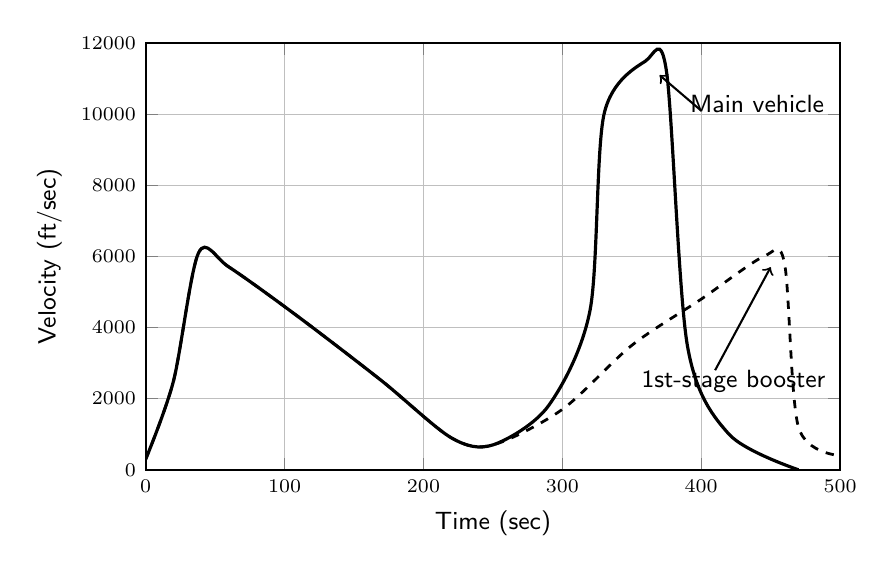
\begin{tikzpicture}
\begin{axis}[
  width=10.4cm,height=7.0cm,
  xmin=0,xmax=500,ymin=0,ymax=12000,
  xtick={0,100,200,300,400,500},
  ytick={0,2000,4000,6000,8000,10000,12000},
  grid=major,
  axis line style={line width=0.8pt},
  tick label style={font=\scriptsize},
  label style={font=\sffamily\small},
  xlabel={Time (sec)},ylabel={Velocity (ft/sec)},
  scaled y ticks=false,
  yticklabel style={/pgf/number format/fixed,/pgf/number format/1000 sep={}},
]
  \addplot[line width=1.15pt,smooth] coordinates {(0,300) (20,2500) (38,6100) (60,5700) (110,4300) (170,2500) (220,900) (250,700) (290,1800) (320,4500) (330,10000) (360,11500) (375,11200) (390,3500) (420,1000) (470,0)};
  \addplot[line width=1.0pt,dashed,smooth] coordinates {(0,300) (20,2500) (38,6100) (60,5700) (110,4300) (170,2500) (220,900) (250,700) (300,1700) (350,3500) (400,4800) (445,6000) (460,5800) (470,1200) (500,400)};
  \node[font=\sffamily\small,anchor=west] at (axis cs:385,10300) {Main vehicle};
  \draw[->,line width=0.75pt] (axis cs:400,10100)--(axis cs:370,11100);
  \node[font=\sffamily\small,anchor=west] at (axis cs:350,2500) {1st-stage booster};
  \draw[->,line width=0.75pt] (axis cs:410,2800)--(axis cs:450,5700);
\end{axis}
\end{tikzpicture}
